% \chapter{Long Title}{Short Title}
% The Long Title will appear on the first page of the chapter.
% The Short Title will appear in the table of contents.
% If the Long Title isn't all that long, you can just call
% \chapter{Long Title}{} and the same title will appear in
% both places.


\chapter{Multivariate moment problems and the Radon transform}{}

\section{Classical and multivariate moment problems}
% Let $f(x)$ be a measurable function on $\RR$. For $k \in \NN_0$, define the $k$th moment of $f$ as
% \[
%   c_k = \int_{-\infty}^\infty f(x)x^k ~dx.
% \]
% The sequence ${(c_k)}_{k \in \NN_0}$ is called a moment sequence or a moment problem, and the function $f$ is called a solution to the moment problem. Loosly speaking a moment problem poses the question: Under given constraints (e.g.\ domain, continuity, etc\ldots), to what extent can one determine the solution $f$ from its moments?
Let $\mu$ be a Borel measure on $\RR$. For $k \in \NN_0$, define the $k$th moment of $\mu$ as
\[
  c_k = \int_{-\infty}^\infty x^k ~d\mu(x)
\]
provided the integral converges. The sequence ${(c_k)}_{k \in \NN_0}$ is called a moment sequence or a moment problem, and the measure $\mu$ is called a solution to the moment problem. Loosly speaking a moment problem poses the question: Under given constraints (e.g.\ measures supported within a fixed subset of $\RR^n$), to what extent can one determine a solution $\mu$ (if one exists) from a moment sequence? 

The classical study of moment problems is divided into three cases depending on the support of $\mu$. In each case there is a standard choice of support, from which general results are often derived by a change of variables.
\begin{enumerate}[label=]
  \item \emph{Markov} (or \emph{Haussdorf}) moment problems within a bounded support.
  \[
    \text{supp}(\mu) \subseteq [0,1]
  \]
  \item \emph{Stieltjes} moment problems within a one-sided infinite support. 
  \[
    \text{supp}(\mu) \subseteq [0,\infty)
  \]
  \item \emph{Hamburger} moment problems within a two-sided infinite support.
  \[
    \text{supp}(\mu) \subseteq \RR
  \]
\end{enumerate}

In some special cases we will denote the moments $c_k$ in a particular form:
\begin{enumerate}
  \item When $\mu$ is absolutely continuous with respect to the Lebesgue measure $dx$, moments can be defined by
  \[
    c_k = \int f(x)x^k dx
  \]
  where $f(x)$ is the density of $\mu$ with respect to $dx$.
  \item When $\mu$ is the Lebesgue measure on a set $A$ of finite measure, moments can be defined by
  \[
    c_k = \int_A x^k dx.
  \]
\end{enumerate}
We often use these representations interchangeably. For example, we may say a function $f$ is determinate, or a set $A$ is indeterminate, if the corresponding measure $\mu$ has that property.

There are two natural questions one can ask about a moment problem:
\begin{itemize}[label=]
  \item \emph{Solvability}: Does a solution $\mu$ exist possessing the given moments?
  \item \emph{Determinacy}: Is a solution unique? If not, what can be said about the set of solutions?
\end{itemize}

For our purposes we will assume existence. In terms of the shape reconstruction method of Chapter 3 it is taken as a given that a solution exists, but that we have access only to the moments. Furthermore in practical application we encounter a followup question to determintacy: How can we reconstruct the solution?

In the classical cases (Markov, Stieltjes, Hamburger) these questions have been more or less resolved. Precise conditions for solvable and determinate moment problems have been found, and the nature of solution sets to indeterminate moment problems are well understood. For instance, all solvable Markov moment problems are unique. This result follows from the Weierstrass approximation theorem:

\begin{proposition}
  All Markov moment problems are determinate. If $\mu, \nu$ are Borel measures on the unit interval $[0,1]$ with equal moments,
  \[
    \int_0^1 x^k d\mu = \int_0^1 x^k d\nu, \qquad k \in \NN_0,
  \]
  then $\mu = \nu$.
\end{proposition}

% \begin{proof}
%   By linearity it is sufficient to show that if $c_k = 0$ for all $k \in \NN_0$, then $\mu = 0$. Furthermore, 
% \end{proof}

\begin{myexample}
  An example of an indeterminate stieltjes moment problem?
\end{myexample}

However, in the case of multivariable moment problems remain largely open. Let $\mu$ be a Borel measure now on $\RR^n$. For $\alpha \in \NN_0^n$. Define the $\alpha$th multivariate moment of $f$ as 
\[
  c_\alpha = \int_{\RR^n} x^\alpha ~d\mu(x).
\]

\begin{myexample}
  Let $A = {[0,1]}^n \subseteq \RR^n$ be the unit cube and $\mu$ the Lebesgue measure on $A$. Then $\mu$ has multivariable moments
  \begin{align*}
    \int_{\RR^n} x^\alpha ~d\mu(x) 
    &= \int_{{[0,1]}^n} x_1^{\alpha_1}x_2^{\alpha_2} \cdots x_n^{\alpha_n} dx \\
    % &= \int_0^1 \int_0^1 \cdots \int_0^1 x_1^{\alpha_1}x_2^{\alpha_2} \cdots x_n^{\alpha_n} ~dx_1~dx_2\cdots~dx_n \\
    &= \int_0^1 x_1^{\alpha_1} ~dx_1 \int_0^1 x_2^{\alpha_2} ~dx_2 \cdots \int_0^1 x_n^{\alpha_n} ~dx_n \\
    &= \frac{1}{(\alpha_1+1) (\alpha_2+1) \cdots (\alpha_n+1)}
  \end{align*}
  Similarly for the Lebesgue measure $\mu$ on any rectanglular region $A = \prod_{i = 1}^n [a_i, b_i]$
  \[
    \int_A x^\alpha ~d\mu(x) 
    = \prod_{i=1}^n \int_{a_i}^{b_i} x_i^{\alpha_i}
    = \prod_{i = 1}^n \frac{b_i^{\alpha_i + 1} - a_i^{\alpha_i + 1}}{\alpha_i + 1}
  \]
\end{myexample}
The moment sequence ${(c_\alpha)}_{\alpha \in \NN_0^n}$ is now multiindexed, but the notions of solvability and determinacy are analogous: It is solvable provided there exists a Borel measure with these moments, and it is determinate provided such a measure is unique. Here, we divide multivariate moment problems into two cases:

\begin{enumerate}[label=]
  \item \emph{Bounded} multivariate moment problems within a bounded support.
  \[
    \text{supp}(\mu) \subseteq {[0,1]}^n
  \]
  % \item \emph{Stieltjes} multivatiate moment problems within a half-plane. 
  % \[
  %   \text{supp}(\mu) \subseteq \RR^{n-1} \times [0, \infty)
  % \]
  \item \emph{Unbounded} multivariate moment problems within an unbounded support.
  \[
    \text{supp}(\mu) \subseteq \RR^n
  \]
\end{enumerate}

While conditions for the solvability or determinacy of multivariate moment problems have been found in certain cases \cn, they are nowhere near as comprehensive as those of classical moment problems. One straightforward, albeit limited, approach is to reduce and $n$-variate moment problem to a set of $n$ univariate moment problems~\cite{Pete82}. For example, we employ this strategy in our proofs of propositions [determinacy for bounded domain and gaussian measures].

As in the classical case of Markov moment problems, determinacy is a consequence of Stone-Weierstrass ($n$-variate polinomials):
\begin{proposition}
  If $\mu$ is a Borel measure on the unit cube $A = {[0,1]}^n$, with moments
  \[
    c_\alpha = \int_{A} x^\alpha d\mu, \qquad \alpha \in \NN_0^n
  \]
  then the moment problem $(c_\alpha)_{\alpha \in \NN_0^n}$ is determinate.
\end{proposition}
We present a simple alternate proof in section 1.4 via the Radon transform.

\begin{myexample}
  An example of an indeterminate, unbounded, multivariable moment problem?
\end{myexample}

\section{Gaussian measures and the Hermite polynomials}
\begin{definition}
  Let $w(p) : \RR \rightarrow \RR$  be the standard Gaussian density on $\RR$,
  \[
    w(p) = \frac1{\sqrt{2\pi}} e^{\frac{-p^2}2}
  \]
  and $w_n(x) : \RR^n \rightarrow \RR$ the standard Gaussian density on $\RR^n$,
  \[
    w_n(x) = {(2\pi)}^{-\frac n2} e^{\frac{-\|x\|^2}2}.
  \]
  Note that $w = w_1$.
\end{definition}

A couple of formulas: First the Gaussian integral,
\[
  \int_{-\infty}^\infty w(p) ~dp = 1.
\]
This can be proven in a number of clever ways.

Second: The derivative
\[
  w'(p) = -pw(p).
\]

Third: The Gaussian function dominates polynomials in the sense that
\[
  \lim_{p \rightarrow -\infty} P(p)w(p) = 0 = \lim_{p \rightarrow \infty} P(p)w(p)
\]
for any polynomial $P$.

\begin{definition}
  The \textit{Gaussian moments} of a function $f: \RR^n \rightarrow \RR$ are
  \[
    c^G_\alpha = \int_{\RR^n} f(x)x^\alpha w(x) ~dx
  \]
  for $\alpha \in \NN_0^n$.
\end{definition}

\begin{myexample}
  Let $f: \RR \rightarrow \RR$ be the constant function $f(p)=1$. The Gaussian moments of $f$, i.e.\ the moments of $w(p)$, are
  \[
    c^G_k 
    = \begin{cases}
        (k-1)!!, & k~\text{even} \\
        0, & k~\text{odd}
    \end{cases}
  \]
  We have already seen $c_0 = 1$. Furthermore it is not hard to see that for odd $k$, 
  \[
    c^G_k = \int_{-\infty}^\infty p^k w(p) ~dp = 0
  \]
  since $p^k w(p)$ is an odd function.

  Now for $\ell = 1, 2, \ldots$, we derive a recurrence formula for $c_{2\ell}$ by integrating by parts
  \begin{align*}
    c^G_{2\ell}
    &= \int_{-\infty}^\infty p^{2\ell} w(p) ~dp \\
    &= -\int_{-\infty}^\infty p^{2\ell-1} \left(-p w(p)\right) ~dp \\
    &= - \left[p^{2\ell-1} w(p)\right]_{-\infty}^\infty + (2\ell-1)\int_{-\infty}^\infty p^{2\ell-2} w(p) ~dp \\
    &= (2\ell-1)c^G_{2\ell-2}.
  \end{align*}
  Thus by induction,
  \[
    c^G_{2\ell} = (2\ell - 1)(2\ell - 3) \cdots c_0 = (2\ell-1)!!.
  \]

  As an alternate derivation, for readers familiar with the gamma function $\Gamma(z) = \int_0^\infty t^{z-1}e^{-t}$ we present the following. Since $p^2\ell w(x)$ is even,
  \begin{align*}
    \int_{-\infty}^\infty p^{2\ell} e^{-\frac{p^2}2} dp 
      &= 2\int_0^\infty p^{2\ell} e^{-\frac{p^2}2} dp 
  \end{align*}
  Now substituting $t = \frac{p^2}2$, whereby $dt = p~dp$,
  \begin{align*}
    2\int_0^\infty p^{2\ell} e^{-\frac{p^2}2} dp 
      % &= 2\int_0^\infty p^{2\ell - 1} e^{-\frac{p^2}2} dt \\
      &= 2^{\ell+\frac12}\int_0^\infty t^{\ell - \frac12}e^{-t} dt \\
      &= 2^{\ell+\frac12} \Gamma\left(\ell + \frac12\right)
  \end{align*}
  so that
  \[
    c^G_{2\ell} = \frac{2^{\ell}}{\sqrt{\pi}} \Gamma\left(\ell + \frac12\right) = (2\ell - 1)!!
  \]
\end{myexample}



A relationship between the univariate and multivariate Gaussian densities can be seen as follows: Let $x, y \in \RR^n$, $n \geq 2$. Suppose $y = p\omega$ where $\omega \in S^1$ and $p \in \RR$, so that $p\omega$ is the orthogonal projection of $x$ onto the span of $y$. Then the Pythagorean relation,
\[
  \|x\|^2 = \|x - p\omega\|^2 + \|p\omega\|^2 = \|x - p\omega\|^2 + p^2
\]
implies that
\begin{align*}
  w_n(x) 
  &= {(2\pi)}^{-\frac n2} e^{\frac{-\|x\|^2}2} \\
  &= {(2\pi)}^{-\frac{n-1}2} e^{\frac{-\|x - p\omega\|^2}2} {(2\pi)}^{-\frac12} e^{\frac{-p^2}2} \\
  &= w_{n-1}(x - p\omega)w(p)
\end{align*}
The equation
\begin{equation}\label{eq:gaussPythag}
  w_n(x) = w_{n-1}(x - p\omega)w(p)
\end{equation}
is in some respect the defining property of the Gaussian measure described below. Indeed if $x = (x_1, x_2, \ldots, x_n)$, by repeated application of (\ref{eq:gaussPythag}) one can write the decomposition
\[
  w_n(x) = \prod_{k = 1}^n w(x_k).
\]
Thus the $w_n(x)$ is the product of $n$ copies of $w$. The standard Gaussian measure $\gamma^n$ is thus a measure whose cardinal projections are standard Gaussian measures.

\begin{definition}
Let $\gamma^n$ be the Borel measure on $\RR^n$ with density $w_n$,
\[
  \int_{\RR^n} f(x) d\gamma^n = \int_{\RR^n} f(x) w_n(x) ~dx.
\]
We call $\gamma^n$ the \textit{standard Gaussian measure}. 
More generally, for mean $a \in \RR^n$, and variance $\sigma > 0$, the following $\gamma^{n}_{a, \sigma^2}$ are \textit{Gaussian measures},
\begin{align*}
  \int_{\RR^n} f(x) d\gamma^n_{a,\sigma^2}
  &= \frac{{(2\pi)}^{-\frac n2}}{\sigma}  \int_{\RR^n} f(x) e^{-\frac{\|x - a\|^2}{2\sigma^2}} ~dx \\
  &= \int_{\RR^n} f(\sigma x + a) d\gamma^n
\end{align*}
% (Most general defn of Gaussian measures includes degenerate $\delta$ functions, and any product of Gaussian measures).
\end{definition}

\begin{myexample}
  Let $f:\RR^n \rightarrow \RR$ be the constant function $f(x)=1$. The Gaussian moments of $f$ are the multivariate moments of $w_n(x)$, and can be written as
  \begin{align*}
    c^G_\alpha 
    &= \int_{\RR^n} x^\alpha w_n(x) ~dx \\
    &= \prod_{\ell = 1}^n \int_{-\infty}^\infty x_\ell^{\alpha_\ell} w(x_\ell) ~dx \\
    &= \prod_{\ell = 1}^n c^G_{\alpha_\ell}
  \end{align*}
  where $\{c_k\}_{k \in \NN}$ are the univariate moments of $w(p)$.
  Thus $c^G_\alpha = 0$ if any $\alpha_i$ is odd. Otherwise, if every $\alpha_i$ is even then
  \[
    c^G_\alpha = \prod_{\ell = 1}^n (\alpha_\ell - 1)!!
  \]
\end{myexample}

% Next we discuss the Hermite polynomials. They can be defined in many equivalent ways, as orthogonal polynomials with respect to the Gaussian weight, as eigenfunctions for 

\begin{definition}
  The \emph{Hermite polynomials} can be defined by the Rodrigues formula
  \[
      H_k(p) = {(-1)}^k \frac{w^{(k)}(p)}{w(p)}
  \]
  
\end{definition}

We can derive a recurrence relation for $H_k$ with some basic differential calculus. First multiplying both sides by $(-1)^k w(p)$, we get
\[
   w^{(k)}(p) = {(-1)}^k w(p)H_k(p)
\]
Now we differentiate both sides 
\[
  w^{(k+1)}(p) 
    = {(-1)}^{k} (-pw(p)H_k(p) + w(p)H_k'(p)) 
    = {(-1)}^{k+1} w(p)(pH_k(p) - H_k'(p))
\]
so that, dividing both sides by ${(-1)}^{k+1} w(p)$, we have
\[
  H_{k+1}(p) = pH(p) - H_k'(p)
\]
Since $H_0(p)$ is trivially the constant $1$ we compute the first handful of polynomials:
\begin{align*}
  H_0(p) &= 1 \\
  H_1(p) &= p \\
  H_2(p) &= p^2 - 1 \\
  H_3(p) &= p^3 - 3p \\
  H_4(p) &= p^4 - 6p^2 + 3 \\
  H_5(p) &= p^5 - 10p^3 + 15p
\end{align*}
Note that each $H_k$ is a monic polynomial of  degree $k$, and $H_k$ is an even (odd resp.) function if $k$ is even (odd resp.).
The Hermite polynomials are mutually orthogonal in the sense that for nonnegative integers $\ell < k$,
\begin{align}\label{eq:HOrth}
  \int_{-\infty}^\infty H_\ell(p) H_k(p) w(p)~dp 
  = 0
\end{align}
To see this, substitute the Rodrigues formula for $H_k$,
\[
  (-1)^k \int_{-\infty}^\infty H_\ell(p) w^{(k)}(p)~dp
\]
and integrate by parts
\begin{align*}
  (-1)^k \left(\left[H_k(p)w^{(k-1)}(p)\right]_{-\infty}^\infty - \int_{-\infty}^\infty H'_\ell(p) w^{(k-1)}(p)~dp\right) \\
  = (-1)^{k-1}\int_{-\infty}^\infty H'_\ell(p) w^{(k-1)}(p)
\end{align*}
where the boundary term $\left[H_k(p)w^{(k-1)}(p)\right]_{-\infty}^\infty$ vanishes because of $w(p)$'s rapid decay at $\pm \infty$. Repeat this process until $H_\ell$ is annihilated.

% \begin{remark}
%   We describe (\ref{eq:HOrth}) in terms of ``orthogonality'' because 
% \end{remark}

The Hermite polynomials form a complete orthogonal basis for $L^2(\RR, w)$, the space of function $f : \RR \to \RR$ for which $\int_{-\infty}^\infty f(p)^2 w(p)~dp < \infty$. This is a Hilbert space with inner product $\langle f, g \rangle = \int_{-\infty}^\infty |f(p)g(p)| w(p)~dp$.
\begin{proposition}
   The linear span of the Hermite polynomials $H_0(p), H_1(p), \ldots$ is dense in $L^2(\RR, w)$.
\end{proposition}

\begin{corollary}
  For any $f \in L^2(\RR)$ the moment problem given by
  \[
    c_n \int_{-\infty}^\infty f(p) w(p) dp
  \]
  is determinate.
\end{corollary}

In the section 1.5 we will make use of a different definition for the Hermite polynomials, as Taylor series coefficients for an exponential generating function.
\begin{lemma}
  The Hermite polynomials have the \emph{generating function},
  \[
    \phi(p) = e^{pt - \frac{t^2}2} 
      = \sum_{k = 0}^\infty \frac{H_k(p)}{k!}t^k.
  \]
  which converges absolutely for all $p, t \in \RR$.
\end{lemma}

\begin{proof}
Note that
\[
  e^{pt - \frac{t^2}2} 
    = \frac{e^{-\frac{(p-t)^2}2}}{e^{-\frac{p^2}2}} 
    = \frac{w(p - t)}{w(p)}
\]
so that the Taylor coefficients are precisely
\[
  \left[\frac{d^k}{dt^k}\frac{w(p - t)}{w(p)}\right]_{t = 0} 
    = (-1)^k \frac{w^{(k)}(p)}{w(p)} = H_k(p).
\]
\end{proof}

We can now define a straight forward multivariate analogue or the 
Hermite polynomials 

\begin{definition}
  For $\alpha \in \NN_0^n$ we define the \emph{multivariate Hermite polynomial} $H_\alpha$ by
\[
  H_{\alpha}(x) = H_{\alpha_1}(x_1) \cdots H_{\alpha_n}(x_n), \qquad x = (x_1, \ldots x_n) \in \RR^n 
\]
\end{definition}

The multivariate Hermite polynomials have many useful properties corresponding to those of the classical polynomials. In particular we have the Rodrigues formula
\[
  H_\alpha(x) 
    = (-1)^{|\alpha|}\frac{D_{\alpha}w_n(x)}{w_n(x)}
\]
where $D_\alpha = \frac{\partial^{\alpha_1 + \cdots + \alpha_n}}{\partial x_1^{\alpha_1} \cdots \partial x_n^{\alpha_n}}$. Just like the classical case, this formula can be used to define $H_\alpha$ as multivariate Taylor coefficients for the generating function:
\[
  \phi(x) = e^{\langle x, y\rangle - \frac{\|y\|^2}2} 
    = \frac{w_n(x - y)}{w_n(x)} 
      = \sum_{\alpha \in \NN_0^n} \frac{H_\alpha(x)}{\alpha!}y^\alpha
\]
which we note is absolutely convergent for all $x, y \in \RR^n$. Here we use the same symbol $\phi$ for the univariate and multivariate generating functions at the risk of confusion. It should be clear from context.

% An interesting formula relating the classical and multivariate Hermite polynomials:
% \[
%   \sum_{|\alpha| = k} \frac{H_\alpha(x)}{\alpha!}y^\alpha 
%     = \frac{H_k\left(\frac{\langle x, y \rangle}{\|y\|}\right)}{k!}|y|^k
% \]
% can be found in a more general form, from Erd\'elyi, Rosier, and others \cn. If $\|y\| = 1$ this says
% \[
%   \sum_{|\alpha| = k} \frac{H_\alpha(x)}{\alpha!}y^\alpha 
%     = \frac{H_k\left(\langle x, y \rangle\right)}{k!}
% \]

% A related formula, assuming $\|y\| = 1$,
% \[
%   \sum_{|\alpha| = k} \frac{H_k(p)}{\alpha!}(y^\alpha)^2
%     = \frac{H_k(p)}{k!}
% \]
% derived independently by Sengupta, looks similar but is very different. z


\section{The Radon and Gaussian Radon transforms}

Let $f$ be a function on the $n$-dimensional Euclidean space $\RR^n$. We imagine taking ``slices'' of $f$ by restricting it to a $(n-1)$-dimensional hyperplane $\Lambda$. These hyperplanes form the domain of the Radon Transform. More precisely, the Radon Transform associates each slice with a corresponding integral
\[
  R_f(\Lambda) = \int_{\Lambda} f(x) ~dx,
\]
which can be thought of as a $(n-1)$-dimensional measurement of $f$. To be more precise we parametrize the collection of hyperplanes $\Lambda$ by normal vector, $\omega \in S^{n-1}$, and (signed) distance from the origin $-\infty < p < \infty$. Indeed any hyperplane can be described in the form $\Lambda = \{x \in \RR^n: \langle x, \omega\rangle = p\}$. As mentioned, there is a slight inconsistency in these definitions where a hyperplane $\Lambda$ can be indexed by both $\langle \omega, x \rangle = p$ and $\langle -\omega, x \rangle = -p$. This difference is inconsequential for our purposes so we choose the latter definition for clarity.

The Radon transform~\cite{Helg65} (RT) is a thing that I will discuss the history of, with references, in this paragraph. The transform gets its name from Johann Radon, whose first defined the transform in the form below in 1917, although a similar transform was introduced by Paul Funk in 1911~\cn. It is interesting to note that the primary application of the RT in medical imaging (CT scans) was not invented for another half century. I can only hope that in 2076 my dissertation will serve as an absorbent coffee coaster for a sleep deprived student.

\begin{definition}
  Let $f$ be a nonnegative measurable function on $\mathbb{R}^n$. The \emph{Radon transform} $R_f : S^{n-1} \times \RR \rightarrow \RR$ of $f$ is a function which, given a unit vector $\omega \in \RR^n$ and $p \in \RR$, is defined as
  \[
    R_f(\omega, p) = \int\mclimits_{\langle x, \omega \rangle = p} f(x) ~dx,
  \]
  provided the integral converges.
\end{definition}

\begin{myexample}
  For computation it is convenient to write the Radon Transform with an explicit isometric parameterization $x(t)$ of the hyperplane $\langle x, \omega\rangle = p$. In particular we note that there exists a map $x : \RR^{n-1} \rightarrow \RR^n$ such that $x(0) = p\omega$ and
  \[
    R_f(\omega, p) = \int_{\RR^{n-1}} f(x(t)) dt.
  \]

  For reference let's specify an hyperplane parameterization for the $n=2$ case. In $\RR^2$ often we identify $\omega$ with the angle $0 \leq \theta < 2\pi$ such that $\omega = (\cos \theta, \sin \theta)$. We define $x(t)$ by
  \begin{align*}
    x(t) = (t \sin \theta + p \cos \theta, -t \cos \theta + p \sin \theta), \qquad -\infty < t < \infty.
  \end{align*}
  It is not difficult to show that $x(0) = p\omega$, $\langle x(t), \omega \rangle = p$, and most importantly
  \[
    R_f(\omega, p) = \int_{-\infty}^\infty f(t \sin \theta + p \cos \theta, -t \cos \theta + p \sin \theta)~dt
  \]
\end{myexample}

\begin{myexample}
  Let $B(r) = \{x : |x| \leq r\} \subseteq \RR^n$ be the ball of radius $r$.
  \[
    R_{B(r)}(\omega, p) = 
    \begin{cases}
      V_{n-1}\left(\sqrt{r^2 - p^2}\right), & |p| \leq r \\
      0 & |p| > r
    \end{cases}    
  \]
  where $V_n(r)$ is the volume of a hypersphere of radius $r$,
  \[
    V_n(r) = \frac{\pi^{n/2}}{\Gamma(\frac n2+1)} r^n.
  \]
  Note that as a bounded domain, we can guarantee $B(r)$ is integrable on all hyperplanes. In fact the RT of any subset of $B(r)$ is sharply bounded by $R_{B(r)} \leq V_{n-1}(r)$. Also note that $B(r)$ is rotation invariant, hence $R_{B(r)}(\omega, p)$ is independent of $\omega$.
  
  \begin{figure}[h]
    \centering
    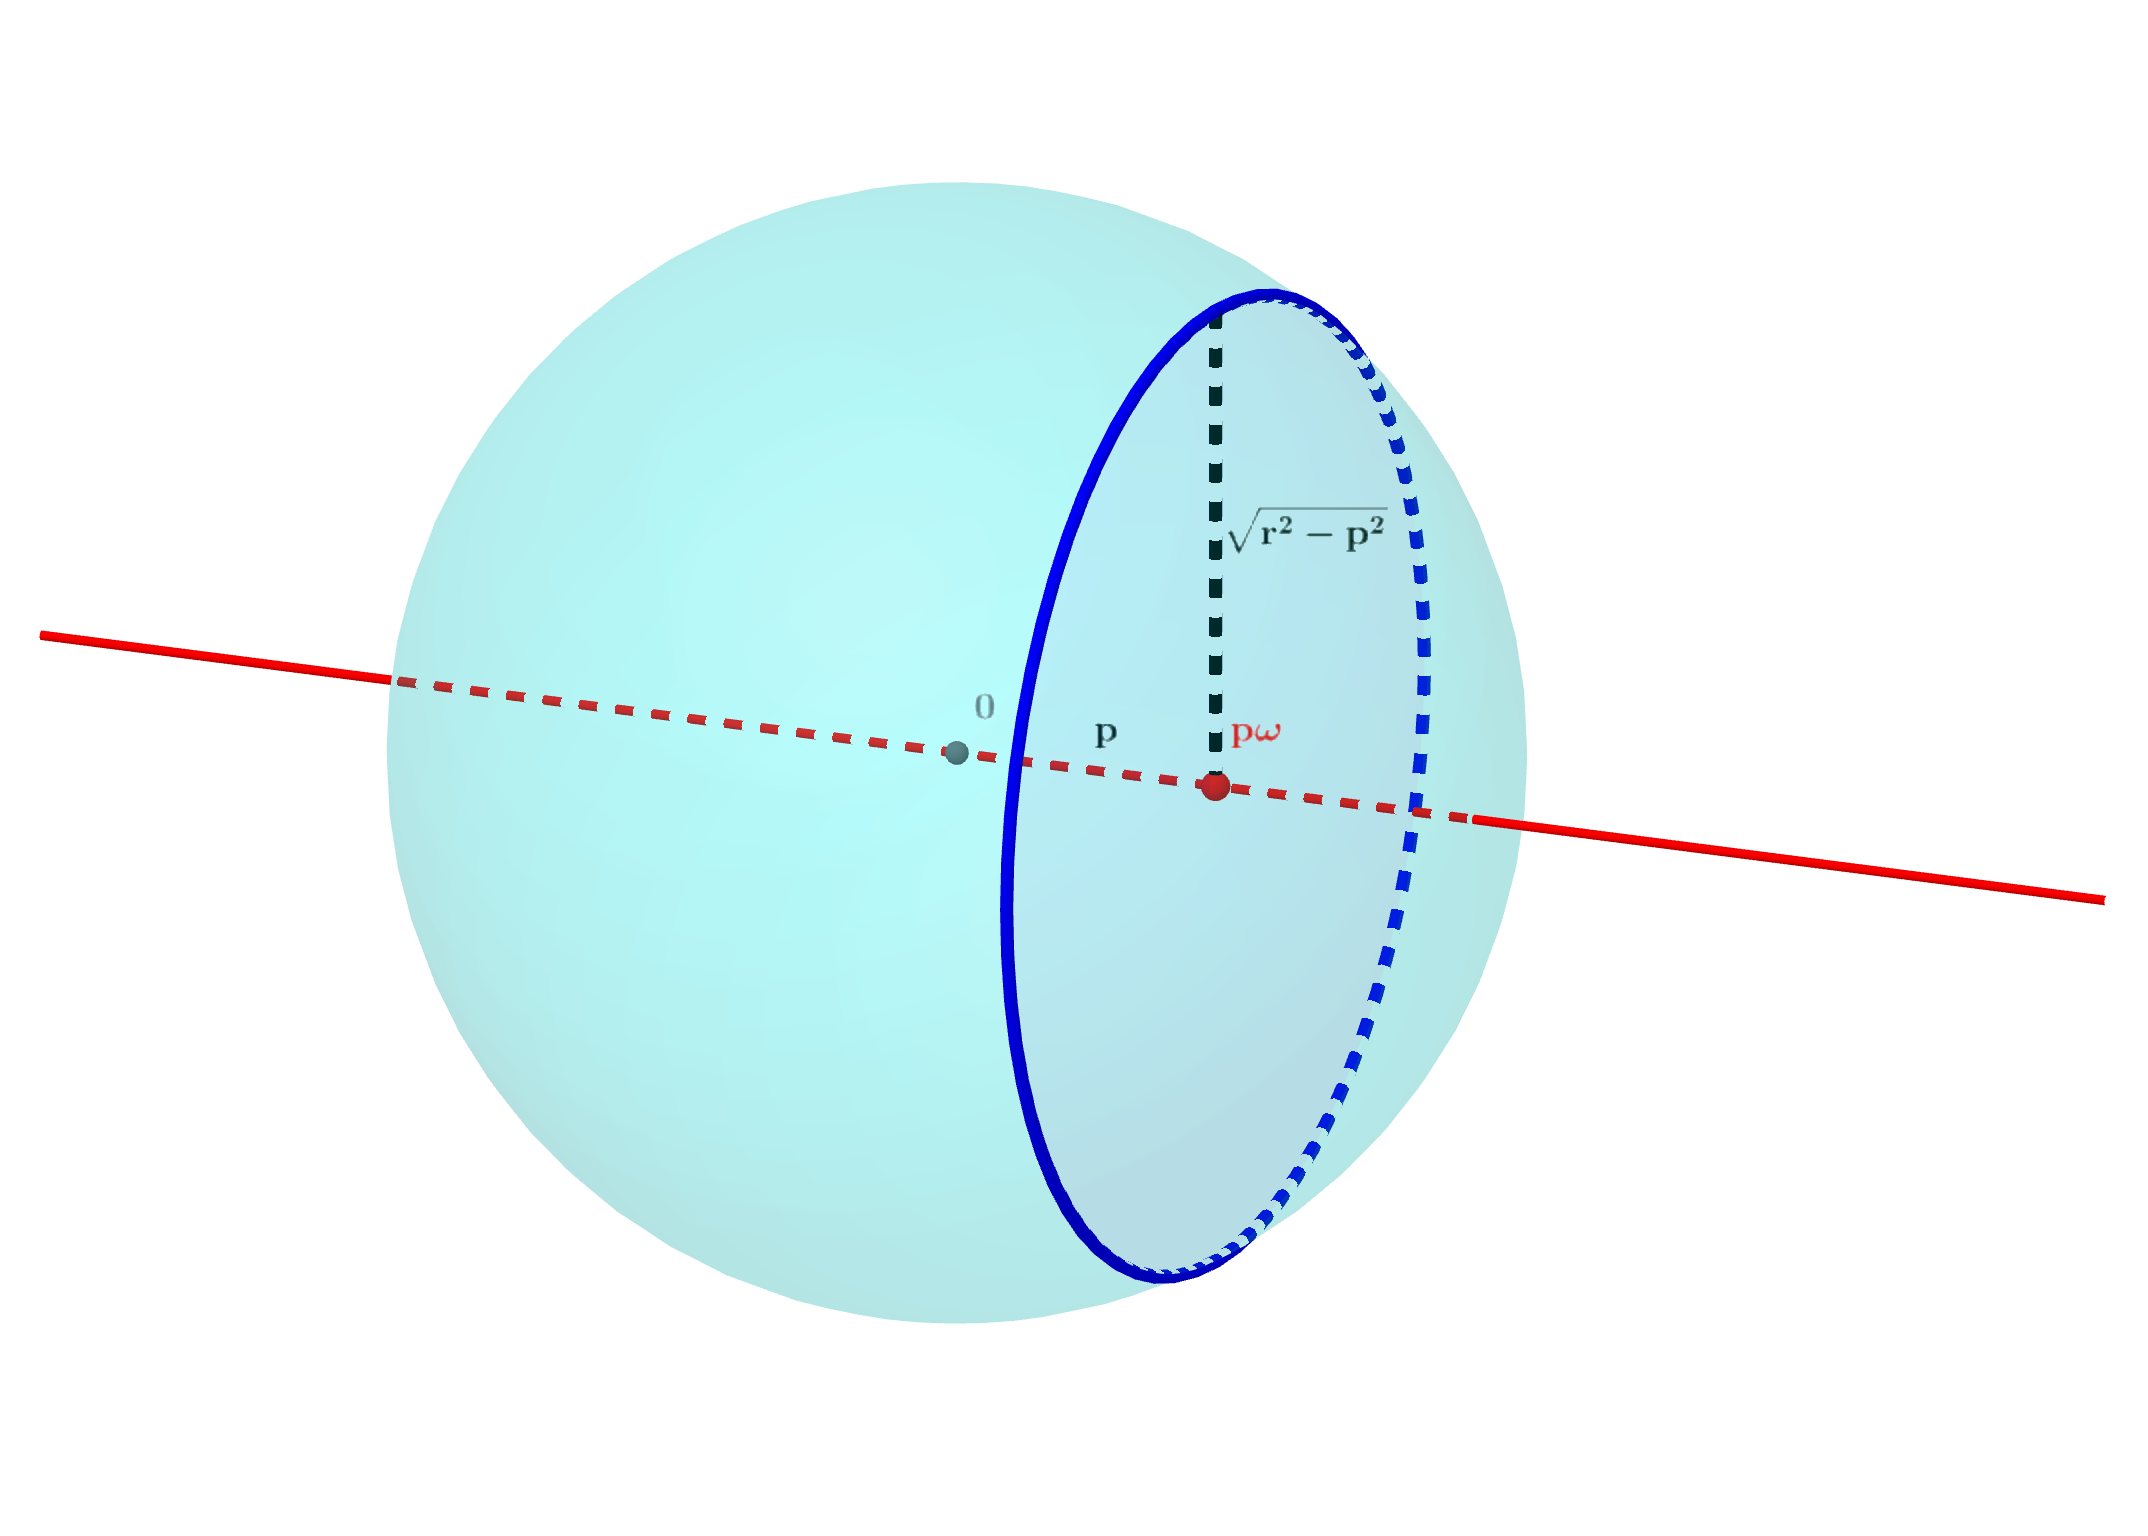
\includegraphics[width=0.7\textwidth]{Images/Ball RT.png}
    \caption{The RT of a ball}\label{fig:RTBall}
  \end{figure}

  We can use this formula to determine the RT of an anulus. Let $A(r_1, r_2) = \{x \in \RR^n: r_1 \leq \|x\| \leq r_2\}$. Then
  \begin{align*}
    R_{A(r_1, r_2)}(\omega, p) 
    &= R_{B(r_2)}(\omega, p) - R_{B(r_1)}(\omega, p) \\
    &= 
    \begin{cases}
      V_{n-1}(\sqrt{r_2^2 - p^2}) - V_{n-1}(\sqrt{r_1^2 - p^2}), & |p| < r_1 \\
      V_{n-1}(\sqrt{r_2^2 - p^2}), & r_1 \leq |p| \leq r_2 \\
      0, & |p| \geq r_2
    \end{cases}
  \end{align*}
\end{myexample}
 


Now consider an example of an unbounded region.

\begin{myexample}
Let $S = \{(x,y) : |y| \leq \frac12\} \subseteq \RR^2$ be a strip centered on the $x$-axis with width $1$. Clearly if $\theta = \pi/2$ or $3\pi/2$ then 
\[
  R_S(\theta, p) = 
  \begin{cases}
      \infty, & |p| \leq \frac12 \\
      0, & |p| > \frac12
  \end{cases}.
\]
Otherwise, 
\[
  R_S(\theta, p) = \sec \theta
\]
Note because $S$ is unbounded, that $R_S$ is not only unbounded, but even divergent in some cases.

\begin{figure}[h]
  \centering
  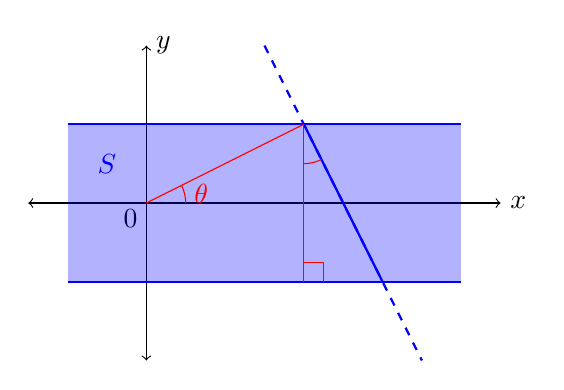
\begin{tikzpicture}[strip/.style={blue, fill=blue, fill opacity = 0.3},
      angle/.style={red},
      axis/.style={<->,black}]
  %draw axes
  \draw[axis] (-1.5,0) -- (4.5,0) node[anchor=west]{$x$};
  \node at (-.2,-.2) {$0$};
  \draw[axis] (0,-2) -- (0,2) node[anchor=west]{$y$};
  %draw wedge
  \fill[strip] (-1, 1) -- (4,1) -- (4, -1) -- (-1, -1) -- cycle;
  \draw[thick, blue] (-1,1) -- (4,1);
  \draw[thick, blue] (-1,-1) -- (4,-1);
  \node[blue] at (-0.5,0.5) {$S$};
  %draw hyperplane
  \draw[thick, blue, dashed] (1.5,2) -- (3.5,-2);
  \draw[thick, blue] (2,1) -- (3,-1);
  %draw angles
  \def\ra{.5};
  \draw[red] (0,0) -- (2,1);
  \draw[red] (\ra,0) arc (0:26.57:\ra) node[midway, right]{$\theta$};
  \draw[red] (2,1) -- (2,-1);
  \draw[red] (2,-1+\ra/2) -- (2+\ra/2,-1+\ra/2) -- (2+\ra/2,-1);
  \draw[red] (2,1-\ra) arc (270:296.57:\ra);
  % \draw[red] (-1,0) arc (180:135:1)node[midway, left]{$\delta$};
  \end{tikzpicture}
  \caption{RT of a strip}\label{fig:strip}
\end{figure}
% More generally, if $S(\varphi, r_1, r_2) = \{(x,y) : r_1 \leq x \cos \varphi + y \sin \varphi \leq r_2\}$ is a strip then (I'm guessing here)
% \[
%     R_{S(\varphi, r_1, r_2)} =
%     \begin{cases}
%         (r_2 - r_1) \sec (\theta - \varphi), & \theta \neq \varphi \pm \frac\pi2 \\
%         \infty, & \theta = \varphi \pm \frac\pi2 \text{ and } p \in [r_1, r_2] \\
%         0, & \theta = \varphi \pm \frac\pi2 \text{ and } p \not\in [r_1,r_2]
%     \end{cases}
% \]
\end{myexample}

Our main addition to previous work will be the use of a modified RT, the Gaussian Radon transform (GRT). This transform is very similar to the RT, but the inclusion of a Gaussian density $w_{n-1}(x)$ in the integral allows for convergence on a larger class of functions $f$. This includes for example unbounded regions. In a broader context the Gaussian Radon transform also has the advantages of generalizng to infite dimensional Hilbert spaces~\cite{Seng14} (on which the Lebesgue measure is not defined), as well as having a natural probabilistic interpretation.

\begin{definition}
The \textit{Gaussian Radon transform} $GR_f : S^{n-1} \times \RR \rightarrow \RR$ of $f$ is defined similarly to the RT.\@ Given $\omega \in S^{n-1}$ and $-\infty < p < \infty$, the GRT is
\[
  GR_f(\omega, p) = 
  \int\mclimits_{\langle x, \omega \rangle = p} f(x) w_{n-1}(x - p\omega) ~dx.
\]
provided the integral converges. Note the Gaussian density 
\[
  w_{n-1}(x - p\omega) = {(2\pi)}^{-(n-1)/2}e^{-\|x - p\omega\|^2/2}
\] 
is centered on the point of the hyperplane closest to the origin.
\end{definition}

\begin{figure}[h]
    \centering
    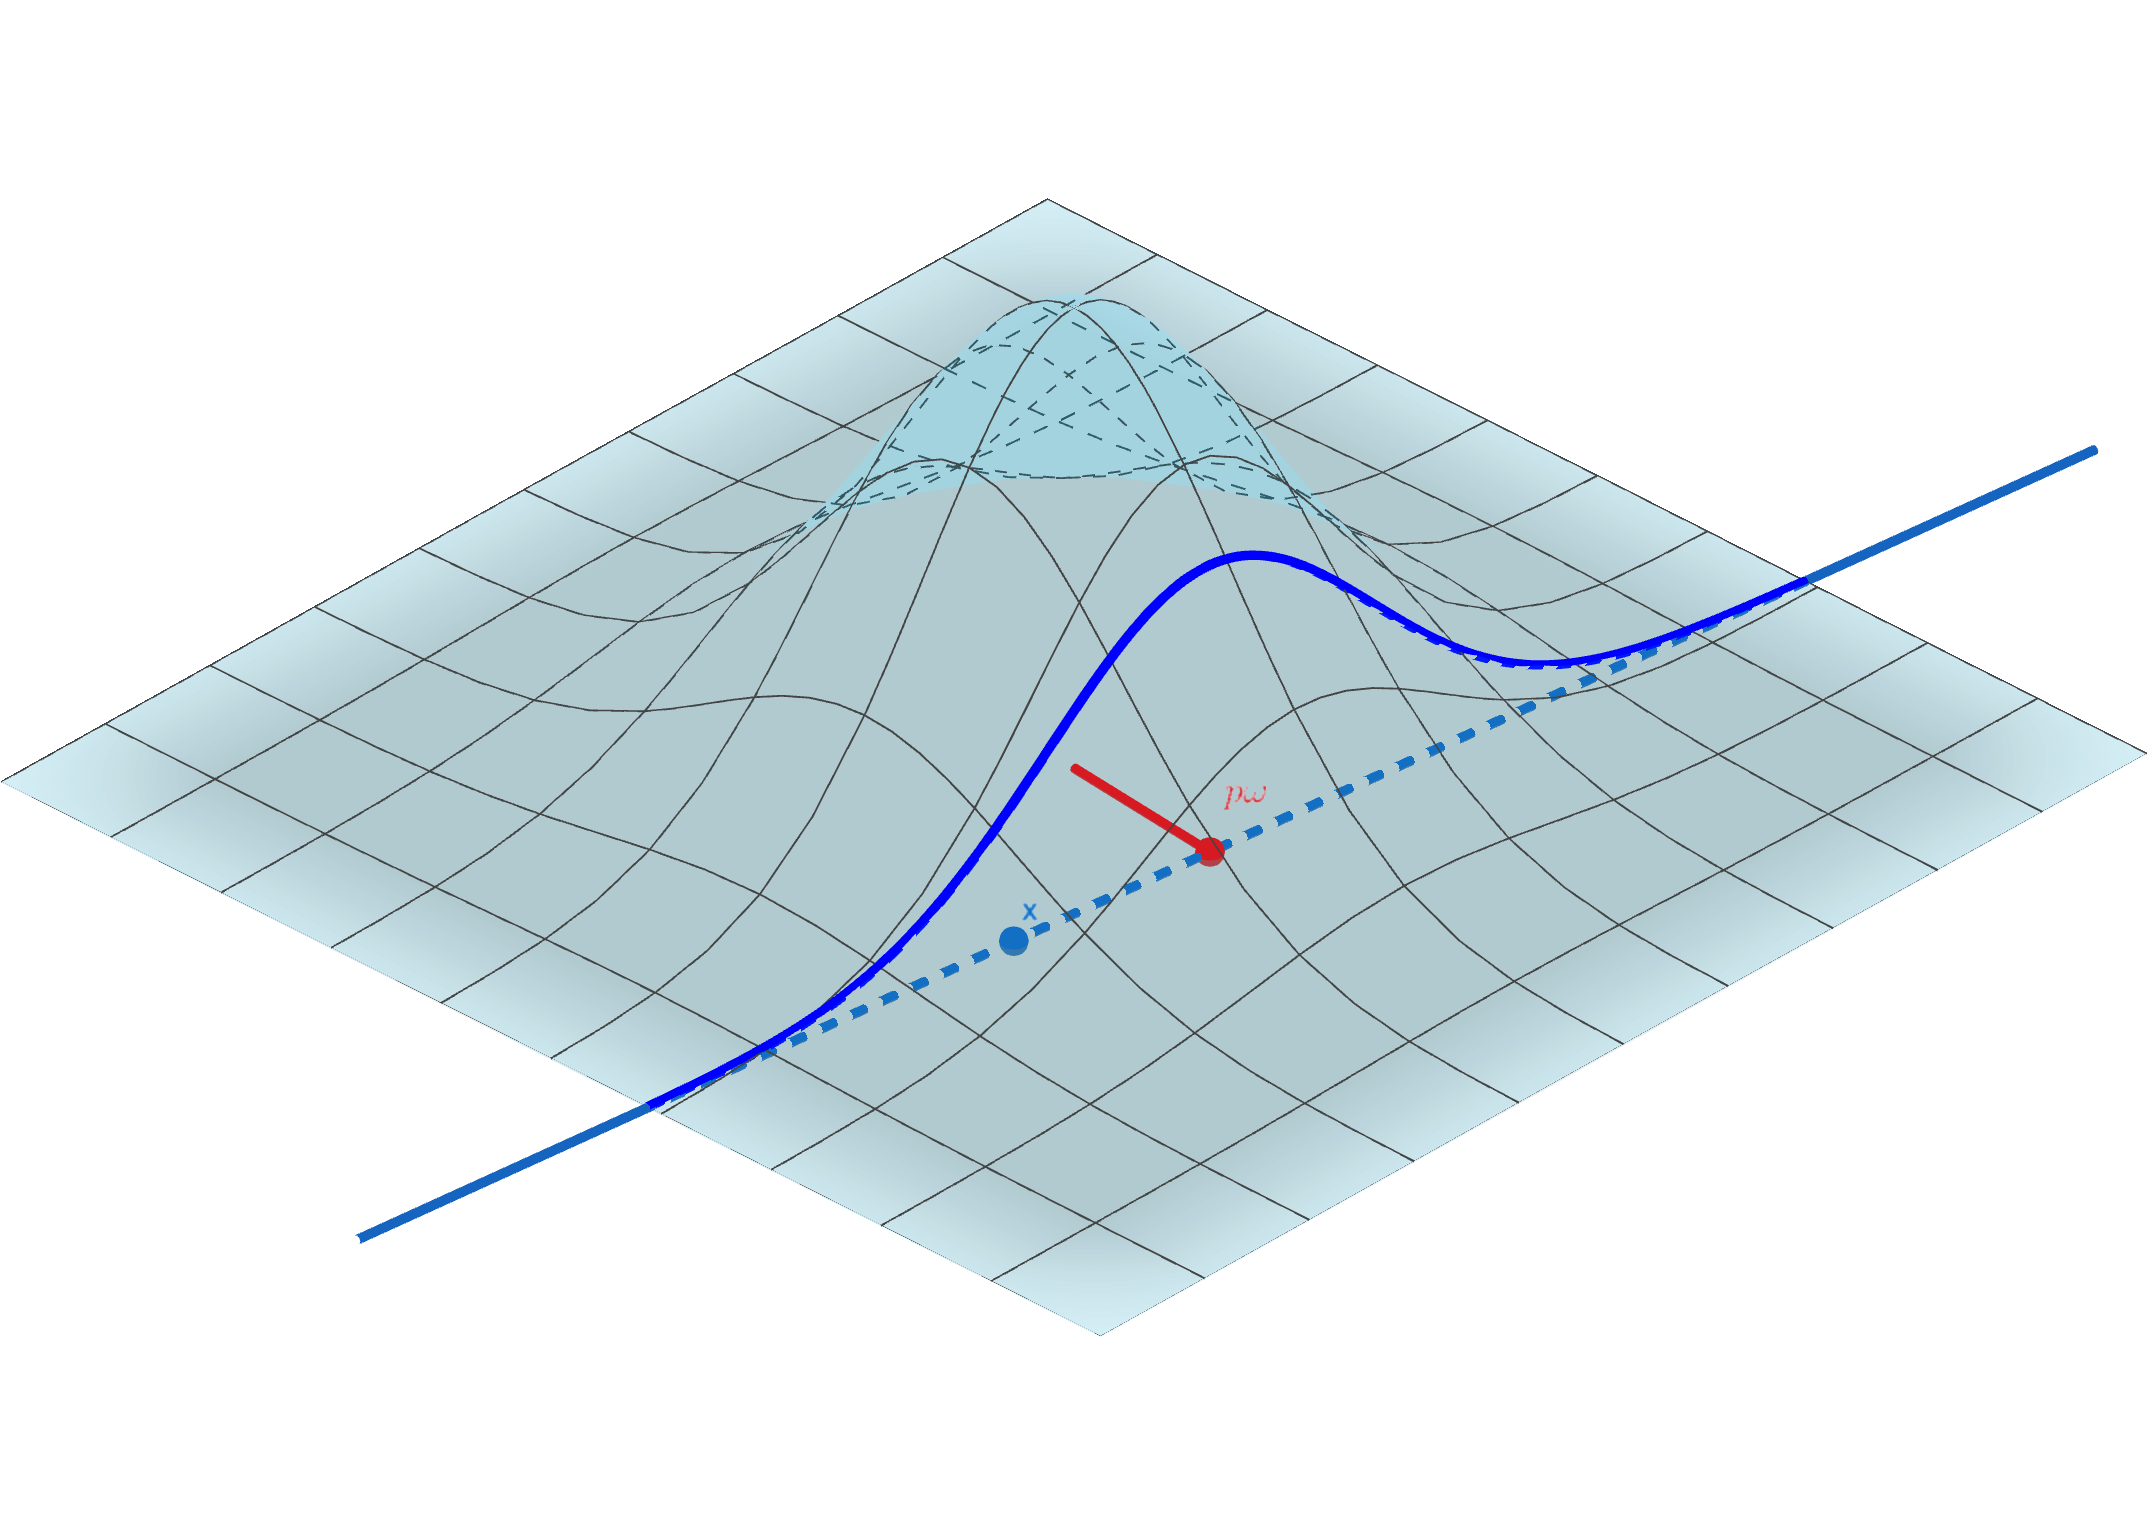
\includegraphics[width=0.7\textwidth]{Images/GRT.png}
    \caption{The GRT}\label{fig:GRT}
\end{figure}

\begin{remark}
  It may be helpful to understand the GRT as a simple modification of the RT with respect to a Gaussian measure on $\RR^n$. From the relation
  \begin{align*}
    \int\mclimits_{\langle x, \omega \rangle = p} f(x) w_n(x) ~dx
    &= \int\mclimits_{\langle x, \omega \rangle = p} f(x) w_{n-1}(x) ~dx~ w(p),
  \end{align*}
  we can express the GRT of $f$ in terms of the $RT$ of the function $g(x) = f(x)w_n(x)$:
  \begin{equation}
    \label{eq:GRTPythag}
    R_g(\omega, p) = GR_f(\omega, p) w(p), \qquad g(x) := f(x)w_n(x).
  \end{equation}
  The relation above provides decent intuition for the GRT, and is also a useful tool proving some basic properties of the transform. Expand on intuition (maybe with example.)
\end{remark}

\begin{myexample}
  If $x(t):\RR^{n-1} \to \RR^n$ is a parametrization of $\langle x, \omega\rangle = p$ as described above, then
  \[
    GR_f(\omega, p) = \int_{\RR^{n-1}}f(x(t)) w_{n-1}(t) dt
  \]
  In particular for $f:\RR^2 \to \RR$
  \[
    GR_f(\omega, p) = \int_{-\infty}^\infty f(t \sin \theta + p \cos \theta, -t \cos \theta + p \sin \theta) w(t)~dt
  \]
  where $\omega = (\cos \theta, \sin \theta)$.
\end{myexample}

\begin{myexample}
  The Gaussian Radon transform is bounded for any measurable region $A \subseteq \RR^n$. Indeed 
  \[
      GR_A(\omega, p) \leq GR_1(\omega, p) = \int_{\RR^{n-1}} w_{n-1}(t)dt w(p) = w(p)
  \]
\end{myexample}

\begin{myexample}
  Consider the Strip $S \subseteq \RR^2$ from [earlier example]. While the RT of $S$ was divergent for $\theta = \pi/2$ or $3\pi/2$, the GRT converges. In particular,
  \[
    GR_S(\theta, p)
    = \begin{cases}
      \frac1{\sqrt{2\pi}}e^{-\frac{p^2}2}, & |p| \leq \frac12 \\
      0, & |p| > \frac12
    \end{cases}
  \]
  This is the density of a ``truncated'' normal distribution on $[-\frac12,\frac12]$. For other angles $GR_S(\theta, p)$ is likewise the density of a truncated normal distribution, this time with arbitrary endpoints $[a, b]$, given by
  \[
    a = ?, \qquad b = a + \sec\theta
  \]
\end{myexample}

Now imagine sweeping a hyperplanar ``slice'' across $\RR^n$. As a function of $p$, $R(\omega, p)$ can be seen as a projection of $f$ onto the linear subspace spanned by $\omega$. It is not surprising that integrating this projection over $-\infty < p < \infty$ we get the same result as the $n$-fold integral of $f$ over $\RR^n$.
\[
    \int_{-\infty}^\infty R(\omega, p) ~dp = \int_{\RR^n} f(x) ~dx
\]
The so called ``slice theorem'' further generalizes this observation:

\begin{proposition}[Slice Theorem]
  % If $f: \RR^n \rightarrow \RR$ and $F: \RR \rightarrow \RR$ are measureable, then
  If $f \in L^1(\RR^n)$ and $F \in L^\infty(\RR)$, then
  % If $f \in C_c(\RR^n)$ and $F \in L^1_{loc}(\RR)$, then
  % \needed{EXTRA CONDITIONS} (i.e. non-negative Fubnini,  Tonelli)
  \begin{align}
    \label{eq:ST}
    \int_{-\infty}^\infty R_f(\omega, p) F(p) dp 
    % &= \int_{-\infty}^\infty \int_{\langle x, \omega \rangle = p} f(x) F(p) ~d\mu(x) ~dp 
    &= \int_{\mathbb{R}^n} f(x) F(\langle x, \omega \rangle) dx,
  \end{align}
  % so long as one of the two is finite.
\end{proposition}

\begin{proof}
  This is a corollary of the Fubini-Tonelli theorem, which guarentees the slice formula as the integrals on eather side converge absolutely. To see this note that there is a rigid transformation (Hilbert space isorphism) taking this to an itterated integral over $\RR^{n-1}$ and $\RR$. Further, $F(\langle x, \omega \rangle) \in L^\infty(\RR^n)$, so the proposition follows by H\"older's inequality
  \[
    \int_{\RR^n} \left|f(x) F(\langle x, \omega \rangle)\right| ~dx \leq \int_{\RR^n}|f(x)| ~dx \|F(\langle x, \omega \rangle)\|_\infty <  \infty
  \] 
  % (under which the Euclidean measures are invariant), the is an integral over $\RR^{n-1}$
  % Fubini's theorem applies since if 
  % Inserting the definition of the RT, the left side is
  % \[
  %   \int_{-\infty}^\infty \int\mclimits_{\langle x, \omega \rangle = p} f(x) ~dx~ F(p) ~dp 
  %   = \int_{-\infty}^\infty \int\mclimits_{\langle x, \omega \rangle = p} f(x) F(\langle x, \omega \rangle) ~dx dp.
  % \]
  % Up to a rigid transformation (under which the Euclidean measures are invariant) this is essentially an itterated integral over $\RR$ and $\RR^{n-1}$. Thus given the integrability requirement, Fubini's theorem applies and the slice theorem is proved.
\end{proof}

\begin{remark}
  % Although we invoke the general Fubini condition here, we note a couple of more convenient sufficient conditions. First, if $f \in L^1(\RR^n)$ and $F \in L^\infty(\RR)$ then,
  The sufficient conditions for the slice theorem above can loosened significantly. We can take for example the straightforward Fubini condition 
  \[
      \int_{\RR^n} |f(x)F(\langle x, \omega \rangle )| < \infty
  \]
  which is necessary \cn, but not convenient. We may also use the condition $f$ has bounded support and $F \in L^1_{loc}(\RR)$.

  The conditions on $f$ and $F$ can be reduced somewhat. In general the convergence of either the left or right side above is sufficient. One 
  % We can specify various conditions for convergence. If $F(p)$ is bounded then $\int |f(x)| dx < \infty$ suffices for convergence. If $f$ is continuous with compact support then $F(p)$ only needs to be integrable.  
\end{remark}

If $F(p) = e^{-ip}$ and $f(x)$ is such that $\int_{-\infty}^\infty R_f(\omega, p) dp < \infty$ then (\ref{eq:ST}) becomes the well known Fourier slice theorem
\[
  \int_{-\infty}^\infty R_f(\omega, p) e^{-ip} ~dp
  = \int_{\mathbb{R}^n} f(x) e^{-i\langle x, \omega\rangle} ~dx,
\]
which is often articulated as saying that the $1$-dimensional Fourier transform of the Radon transform is the $n$-dimenstional Fourier transform of $f$.

An early and natural question in the study of the RT is that of inversion. Radon himself derived the ``Radon inversion formula''~\cite{Rado17}~\cite{Rado86}, which is often proved via the above Fourier slice theorem. The groundbreaking inversion formula is the basis for what, in application, called ``filtered backpropogation''.

If one is interested in inverting the RT then a prerequisite concern is of course: Is the transform injective? The answer clearly depends on what space we draw the function $f$ from. Radon~\cite{Rado17}~\cite{Rado86} provides a set of sufficient regularity conditions such that the RT is invertible. Other similar results followed \cite{????}. On the other hand counterexamples have been constructed by, for example, Lawrence Zalcman~\cite{Zalc82}, of continuous and nontrivial functions for which the RT is identically zero.

By way of the relation (\ref{eq:GRTPythag}) we can prove an analogous slice theorem for the GRT.\@ Mihai and Sengupta prove the general result if real, separable, infinite Hilbert spaces \cn.

\begin{proposition}[Gaussian Slice Theorem] 
  Let $f:\RR^n \rightarrow \RR$ and $F:\RR \rightarrow \RR$ be measurable functions. If $f \in L^1(\RR^n, w_n)$ and $F \in L^\infty(\RR)$ then
  \begin{equation}\label{eq:GST}
    \int_{-\infty}^\infty GR_f(\omega, p)F(p) w(p) ~dp
    = \int_{\mathbb{R}^n}f(x) F(\langle x, \omega\rangle) w_n(x) ~dx. 
  \end{equation}
\end{proposition}

\begin{remark}
  Again the more general Fubini condition
  \[
    \int_{\mathbb{R}^n} |f(x) F(\langle x, \omega\rangle) w_n(x)| dx < \infty
  \]
  may be used. Further, whatever conditions on $f$ and $F$ are sufficient for convergence in (\ref{eq:ST}) are then sufficient conditions to be checked of $f(x)w_n(x)$ and $F(p)w(p)$. I'll need to check these conditions more carefully.
\end{remark}



\begin{proof}
  From (\ref{eq:GRTPythag})
  \[
    \int_{-\infty}^\infty GR_f(\omega, p)F(p) w(p) ~dp 
    = \int_{-\infty}^\infty R_g(\omega, p) F(p) ~dp
  \]
  where $g(x) = f(x)e^{-\|x\|^2/2}$. Note that $\|g\|_1 = \|f\|_{1,w_n} < \infty$ and. Then applying the slice theorem:
  \[
    \int_{-\infty}^\infty R_g(\omega, p) F(p) ~dp 
    = \int_{\RR^n} f(x)F(\langle x, \omega \rangle) w_n(x) ~dx,
  \]
  completing the proof.
\end{proof}

% \begin{remark}
%     For an equivalent 
% \end{remark}

\section{The Radon transform of measures}

% Here we extend the definitions of the RT and GRT to apply to 

Taking from the context of classical moment problems we should define the notion of the Radon transform of a measure $\mu$. Let $\mu$ be a Borel measure on $\RR^n$ with finite moments $c_\alpha$, $\alpha \in \NN_0^n$. The projection $\pi_\omega : \RR^n \rightarrow \RR$ given by
\[
  \pi_\omega(x) = \langle x, \omega \rangle
\] 
is a Borel function, thus we may define the push-forward measure $\mu_\omega = \mu \circ \pi_\omega^{-1}$ which for Borel sets $A \subseteq \RR$ is given by,
\[
  \mu_\omega(A) = \mu(\pi_\omega^{-1}(A)) = \mu(\{x : \langle x, \omega \rangle \in A\}).
\]
We may call $\mu_\omega$ the \emph{marginal projection measure} of $\mu$ with direction vector $\omega$.

Notice that if $\mu$ is absolutely continuous with density representation $\mu = f(x)dx$ then the slice theorem with $F(p)$ the characteristic function of $A$ gives,
\[
  \mu(\pi_\omega^{-1}(A)) = \int\mclimits_{\langle x, \omega \rangle \in A} f(x)dx = \int_A R_f(\omega, p) dp
\]
so that in fact $\mu_\omega$ is absolutely continuous with respect to the Lebesgue measure $dp$ and it's density is precisely the Radon transform $R_f(\omega, p)$. In this sense the marginal projection $\mu_\omega$ is a natural generalization of the RT, so we define

\begin{definition}
  The Radon transform of a Borel measure $\mu$ on $\RR$ is defined as the push-forward measure $\mu_\omega = \mu \circ \pi_\omega^{-1}$ on $\RR$, where $\pi_\omega: \RR^n \rightarrow \RR$ is the projection 
  \[
    \pi_\omega(x) = \langle x, \omega \rangle.
  \]
  We may denote this measure by $R_\mu^\omega = \mu_\omega$.
\end{definition}

\begin{remark}
  It seems that the slice theorem is analogous to — and perhaps generalized by — the change of variables formula for the pushforward measure $R^\omega_\mu$:
  \[
    \int_{-\infty}^\infty F(p) dR^\omega_\mu(p) = \int_{\RR^n} F(\pi_\omega(x)) d\mu
  \]
  where $F:\RR \rightarrow \RR$ is integrable with respect to $dR^\omega_\mu$ if and only if $F\circ\pi_\omega : \RR^n \rightarrow \RR$ is integrable with respct to $\mu$.
\end{remark}
Can we similarly define the GRT of a measure?

\begin{proposition}
  Let $c_\alpha (\omega) = \int_{-\infty}^\infty R_f(\omega, p) p^k dp$ be the projection moments of $f$ at a fixed $\omega$, and $c_\alpha$ the multivariate moments of $f$. Then
  \[
      c_k(\omega) = \sum_{|\alpha| = k}\binom{k}{\alpha} \omega^\alpha c_\alpha
  \]
  where $\binom{k}{\alpha} = \frac{k!}{\alpha_1! \alpha_2! \cdots \alpha_n!}$ are multinomial coefficients.
\end{proposition}

\begin{proof}
  By the slice theorem (\ref{eq:ST}) with $F(p) = p^k$,
  \[
    \int_{-\infty}^\infty R_f(\omega, p) p^k ~dp 
    = \int_{\RR^n} f(x) \langle x, \omega \rangle^k ~dx.
  \]
  Now $\langle x, \omega \rangle^k = {(x_1 \omega_1 + \cdots + x_n \omega_n)}^k$ has the multinomial expansion
  \[
    \langle x, \omega \rangle^k = \sum_{|\alpha| = k}\binom{k}{\alpha} x^\alpha\omega^\alpha.
  \]
  Thus after a bit of rearranging we get
  \begin{align*}
    \int_{\RR^n} f(x) \langle x, \omega \rangle^k ~dx
    &= \int_{\RR^n} f(x) \sum_{|\alpha| = k}\binom{k}{\alpha} x^\alpha \omega^\alpha ~dx \\
    &= \sum_{|\alpha| = k}\binom{k}{\alpha} \omega^\alpha \int_{\RR^n} f(x) x^\alpha ~dx,
  \end{align*}
  where the integrands are precisely the $k$th degree multivariate moments of $f$.
\end{proof}

Similarly, moments of the GRT (Gaussian projection moments) can be expressed in terms of multivariate gaussian moments.

\begin{proposition}
  Let $c_k^G(\omega) = \int_{-\infty}^\infty GR_f(\omega, p) p^k w(p) dp$ be the Gaussian moments of the GRT of $f$ at a fixed $\omega$. Let $c^G_\alpha = \int_{\RR^n} f(x) w_n(x) x^\alpha dx$ be the Gaussian multivariate moments of $f$. Then
  \[
    c^G_k(\omega) = \sum_{|\alpha| = k}\binom{k}{\alpha} \omega^\alpha c^G_\alpha.
  \]
\end{proposition}


\begin{proof}
  The proof follows as it did for the RT.\@ This time we apply the GRT slice theorem (\ref{eq:GST}) with $F(p) = p^k$, 
  \begin{align*}
    \int_{-\infty}^\infty GR_f(\omega, p) p^k w(p) ~dp
    &= \int_{\RR^n} f(x) \langle x, \omega \rangle^k w_n(x) ~dx
  \end{align*}
  Again we use the multinomial expansion of $\langle x, \omega\rangle^n$ and rearange:
  \[
    \int_{\RR^n} f(x) \langle x, \omega \rangle^k w_n(x) ~dx
    = \sum_{|\alpha| = k} \binom{k}{\alpha} \omega^\alpha \int_{\RR^n} f(x) w_n(x)x^\alpha dx. 
  \]
  Thus
  \[
    c^G(\omega) = \sum_{|\alpha| = k} \binom{k}{\alpha} \omega^\alpha c^G_\alpha.
  \]
\end{proof}

\begin{myexample}
  Let $e_1, e_2, \ldots, e_n \in S^{n-1}$ be the the standard basis for $\RR^n$,
  \[
    (1, 0, \ldots, 0),~ (0, 1, \ldots, 0),~ \ldots,~ (0,0, \ldots, 1)
  \]
  Then $\langle x, e_i \rangle = x_i$ is the natural projection of $\RR^n$ onto the $e_i$ axis. The standard projection moments can be calculated as follows
  \begin{align*}
    c_k(e_i) 
    &= \sum_{|\alpha| = k} \binom{k}{\alpha} e_i^\alpha c_\alpha \\
    &= c_{ke_i}
  \end{align*}
  since $e_i^\alpha = 0$ unless $\alpha = ke_i$.
\end{myexample}

The following theorem, due to Petersen \cn, gives a way us to reduce the question of determinacy for multivariate moment problems to the classical case.

\begin{proposition}[Petersen's theorem]
  Let $\mu$ be a Borel measure with finite moments on $\RR^n$, and $e_1, \ldots, e_n$ the standard basis for $\RR^n$. If each $R_\mu^{e_1}, \ldots, R_\mu^{e_n}$ is determinate, then $\mu$ is determinate.
\end{proposition}

\begin{proof}
  An outline of the proof is as follows. Preliminarily, note that the solution set $[\mu]$ of Borel measures with equivalent moments to $\mu$ is convex \cn, and a $\mu$ is an extreme point in $[\mu]$ if and only if polynomials are dense in $L^1(\RR^n, \mu)$ \cn. Thus it suffices to show that polynomials are dense in $L^1(\RR^n, \mu')$ for any $\mu' \in [\mu]$.
  
  The family of products of continuous functions of compact support $f(x) = \prod_{i=1}^n f_i(x_i)$ where each $f_i \in C_c(\RR)$, is dense in $L_1(\mu)$ \cn. Furthermore, since $R_\mu^{e_i}$, $i = 1, \ldots, n$ are determinate, polynomials are dense in each $L^2(\RR, R_\mu^{e_i})$ \cn. Petersen constructs a series of polynomials $P_i : \RR \rightarrow \RR$ such that the polynomial product $P(x) = \prod_{i = 1}^n P_i(x_i)$ arbitrarily close to $f$ in $L^1(\mu)$. Thus polynomials are dense in $L^1(\RR^n, \mu)$ and the moment problem is determinate. \pn 
  
  Note Schm\"udgen proves this via Borel characteristic functions. Not clear what the benefit is.
\end{proof}

\begin{remark}
  Conjecture? We expect this result to hold true for any orthonormal basis, and likely any basis. Will have to check this. Arguable benefit for us is that we in theory can use any $n$ linearly independent projections to reconstruct $\mu$.
\end{remark}

\begin{corollary}
  If $\mu$ is compactly supported Borel measure on $\RR^n$, then the multivariate moment problem is determinate.
\end{corollary}

\begin{proof}
  It suffices to note that the projections $R_\mu^{e_i}$ are compactly supported Borel measures on $\RR$, and thus determinate by \cn.
\end{proof}


We show in section (2.2) that any function $f$ in the weighted space $L^2(\RR, \gamma)$ is determinate (maybe this should be moved to section 1.2). Petersen's theorem allows us to generalize this result to $\RR^n$.

\begin{corollary}
  If $f \in L^2(\RR^n, \gamma^n)$, then $f$ is determinate.
\end{corollary}

\begin{proof}
  % This follows from the product decomposition of the the Gaussian density
  % \[
  %   w_n(x) = \prod_{i = 1}^n w(x_i)
  % \]
  % so that
  % \[
  %   R_f(e_i, p) = \int_{x_i=p} f(x) w_n(x) dx
  % \]
  \pn
\end{proof}

\section{The Radon transform of multivariate Hermite polynomials over general affine subspaces}

% The goal of this section will be to explore the generalizations of the RT and GRT as functions of general affine subspaces. We discuss the analogues of many of the previous results in this context.
We begin this section by proving a formula for the GRT of the multivariate Hermite polynomials defined in the previous section. Recall that for $\alpha \in \NN_0^n$ the polynomials $H_\alpha(x)$ can be defined by the generating function
\[
  e^{\langle x, y\rangle - \frac{\|y\|^2}2} = \sum_{\alpha \in \NN_0^n} \frac{H_\alpha(x)}{\alpha!} y^\alpha
\]
where $\alpha! = \alpha_1! \cdots \alpha_n!$. These are related to the classical Hermite polynomials by
\[
  H_\alpha(x) = \prod_{i=1}^n H_{\alpha_i}(x_i)
\]
where, for $k \in \NN_0^\infty$, the classical polynomials $H_{k}(p)$ can be defined by
\[
  e^{pt - \frac{t^2}2} = \sum_{k = 0}^\infty \frac{H_k(p)}{k!}t^k.
\]

\begin{proposition} \label{prop:GRTHermite}
  Let $\omega \in S^{n-1}$ and $p \in \RR$ be fixed. If $|\alpha| = k$, then the GRT of the multivariate Hermite polynomial $H_\alpha$ is
  \begin{equation}\label{eq:GRH}
    GR_{H_\alpha}(\omega, p) = H_k(p)\omega^\alpha
  \end{equation}
\end{proposition}

\begin{proof}
  Recall that the generating function $\phi(x) = e^{\langle x, y\rangle - \frac{\|y\|^2}2}$ converges absolutely for all $x,y \in \RR^n$. Consider the GRT of $\phi$,
  \begin{align*}
    GR_{\phi}(\omega, p) 
      &= \int\mclimits_{\langle x, \omega \rangle = p} \phi(x) w_{n-1}(x - p\omega)~dx.
    % \\&= \int\mclimits_{\langle x, \omega \rangle = 0} \phi(x + p\omega) w_{n-1}(x)~dx
  \end{align*}
  Immediately we can expand $\phi(x)$, interchanging integral and series, to see
  \begin{equation} \label{eq:GRTPhiExpansion1}
    \begin{split}
      GR_{\phi}(\omega, p)
        &= \sum_{\alpha \in \NN_0^n} \frac1{\alpha!} y^\alpha \int\mclimits_{\langle x, \omega\rangle = p} H_\alpha(x) w_{n-1}(x - p\omega)~dx
      \\&= \sum_{\alpha \in \NN_0^n} \frac{GR_{H_\alpha}(\omega, p)}{\alpha!} y^\alpha.
    \end{split}
  \end{equation}
  On the other hand, we will be able to show that
  \begin{equation} \label{eq:GRTPhiExpansion2}
    GR_{\phi}(\omega, p) 
    = \sum_{k = 0}^\infty \sum_{|\alpha| = k} \frac{H_k(p)\omega^\alpha}{\alpha!} y^\alpha.
  \end{equation}
  Thus, being careful to note that the series (\ref{eq:GRTPhiExpansion1}) and (\ref{eq:GRTPhiExpansion2}) converge absolutely, we can compare coefficients for the desired formula. In order to derive the second expansion we begin by translating our integral onto the linear subspace $\langle x, \omega\rangle = 0$, via the change of variables $x \mapsto x + p\omega$:
  \begin{equation}\label{eq:GRTPhiExpansion21}
    \begin{split}
      GR_{\phi}(\omega, p) 
        &= \int\mclimits_{\langle x, \omega\rangle = 0} \phi(x + p\omega) w_{n-1}(x) ~dx 
      \\&= \int\mclimits_{\langle x, \omega\rangle = 0} e^{\langle x + p\omega, y \rangle - \frac{\|y\|^2}2}(2\pi)^{-\frac{n-1}2}e^{-\frac{\|x\|^2}2} ~dx
      \\&= e^{p \langle \omega, y\rangle - \frac{\|y\|^2}2} \int\mclimits_{\langle x, \omega\rangle = 0}e^{\langle x, y\rangle - \frac{\|x\|^2}2} (2\pi)^{-\frac{n-1}2} ~dx
    \end{split}
  \end{equation}
  Now in order to compute the right side integral we consider the orthogonal decomposition $y = y_\omega + y_{\omega^\perp}$, where
  \[
    y_\omega = \langle y, \omega \rangle \omega \qquad y_{\omega^\perp} = y - y_\omega.
  \]
  We make two observations about this decomposition of $y$: First, 
  \begin{equation}\label{eq:GRTPhiExpansion22}
    \|y\|^2 
      = \|y_\omega\|^2 + \|y_{\omega^\perp}\|^2 
      = \langle y, \omega\rangle^2 + \|y_{\omega^\perp}\|^2
  \end{equation}
  and second, for $x$ in the linear subspace $\langle x, \omega\rangle = 0$ we have
  \[
    \langle x, y \rangle
      = \langle x, \omega \rangle \langle y, \omega \rangle + \langle x, y_{\omega^\perp} \rangle 
      = \langle x, y_{\omega^\perp} \rangle.
  \]
  This second observation allows us to solve the integral at the end of (\ref{eq:GRTPhiExpansion21}). By completing the square $\|x - y_{\omega^\perp}\| = \|y_{\omega^\perp}\|^2 - 2\langle x, y_{\omega^\perp} \rangle + \|x\|^2$, we have
  \begin{align*}
    \int\mclimits_{\langle x, \omega\rangle = 0}e^{\langle x, y\rangle - \frac{\|x\|^2}2} (2\pi)^{-\frac{n-1}2} ~dx
      &= e^{-\frac{\|y_{\omega^\perp}\|^2}2} \int\mclimits_{\langle x, \omega\rangle = 0}e^{-\frac{\|y_{\omega^\perp}\|^2}2 + \langle x, y_{\omega^\perp}\rangle - \frac{\|x\|^2}2} (2\pi)^{-\frac{n-1}2} ~dx
    \\&= e^{-\frac{\|y_{\omega^\perp}\|^2}2} \int\mclimits_{\langle x, \omega\rangle = 0}e^{-\frac{\|x - y_{\omega^\perp}\|}2} (2\pi)^{-\frac{n-1}2} ~dx
    % \\&= e^{-\frac{\|p_{\omega^\perp}\|^2}2}
  \end{align*}
  which is just $e^{-\frac{\|p_{\omega^\perp}\|^2}2}$. It was important here to invoke the orthogonal projection $y_{\omega^\perp}$ so that the integrand becomes the translation of a standard Gaussian function on the hyperplane $\langle x, \omega \rangle = 0$. Now returning to (\ref{eq:GRTPhiExpansion21}), we have
  \begin{align*}
    GR_{\phi}(\omega, p) 
      &= e^{p \langle \omega, y\rangle - \frac{\|y\|^2}2-\frac{\|y_{\omega^\perp}\|^2}2}
    \\
      &= e^{p \langle \omega, y\rangle - \frac{\langle y, \omega\rangle^2}2}
  \end{align*}
  where we used (\ref{eq:GRTPhiExpansion22}). This looks like the generating function for the univariate Hermite polynomials $H_k(p)$ with $t = \langle \omega, y \rangle$, so we expand
  \begin{align*}
    GR_{\phi}(\omega, p) 
      &= \sum_{k = 0}^\infty \frac{H_k(p)}{k!} \langle \omega, y\rangle^k.
  \end{align*}
  Finally we apply the multinomial expansion of $\langle \omega, y\rangle^k$, recalling the multinomial coefficients $\binom{k}{\alpha} = \frac{k!}{\alpha!}$. Therefore
  \begin{align*}
    GR_{\phi}(\omega, p)
      &= \sum_{k = 0}^\infty \sum_{|\alpha| = k} \frac{H_k(p)}{k!} \binom{k}\alpha y^\alpha\omega^\alpha
    \\
      &= \sum_{k = 0}^\infty \sum_{|\alpha| = k} \frac{H_k(p)\omega^\alpha}{\alpha!} y^\alpha
  \end{align*}
  as needed.
\end{proof}

\begin{remark}
  The proof above was written by Dr. Sengupta. Recall that the Hermite polynomials $H_\alpha$ form a complete orthogonal basis for $L^2(\RR^n, w_n)$. In this sense the formula (\ref{eq:GRH}) completely defines the Gaussian Radon transform on this space. Indeed, it can be shown that any function $f \in L^2(\RR^n, w_n)$ has an expansion
  \[
    f(x) = \sum_{\alpha \in \NN_0^n} a^{(f)}_\alpha H_\alpha(x)
  \]
  where
  \[
    a_\alpha^{(f)} = \int_{\RR^n} f(x)H_\alpha(x) w_n(x) ~dx.
  \]
  If this expansion converges nicely on $\Lambda$ then
  \begin{align*}
    GR_f(\Lambda) 
    &= \int_\Lambda f(x) w_n(x-p_0)~dx 
    \\ 
    &= \int_\Lambda \sum_{\alpha \in \NN_0^n} a_\alpha^{(f)} H_\alpha(x) w_n(x-p_0) ~dx
    \\
    &= \sum_{\alpha \in \NN_0^n} a_\alpha^{(f)} \int_\Lambda H_\alpha(x) w_n(x-p_0) ~dx
    \\
    &= \sum_{\alpha \in \NN_0^n} a_\alpha^{(f)} GR_{H_\alpha}(\Lambda)
  \end{align*}
  If $\Lambda$ is a hyperplane $\inner{x, \omega} = p$ with $\omega \in S^{n-1}$ then this gives
  \begin{align*}
    GR_f(\Lambda) 
    &= \sum_{\alpha \in \NN_0^n} a_\alpha^{(f)} GR_{H_\alpha}(\Lambda)
    \\
    &= \sum_{\alpha \in \NN_0^n} a_\alpha^{(f)} H_{|\alpha|}(p) \omega^\alpha
    \\
    &= \sum_{k=0}^\infty H_k(p) \sum_{|\alpha| = k} a_\alpha^{(f)} \omega^\alpha
  \end{align*}
  For details on modes convergence see (Dunkl or Thangavelu) \cn. 
\end{remark}

In section 1.4 we defined the RT and GRT as the integrals of a function $f: \RR^n \rightarrow \RR$ over $n-1$ dimensional hyperplanes, the standard definitions. But there are many examples of geometric integral transforms, closely related to the hyperplane RT, which can be thought of as ``generalized Radon transforms''. In fact, the ``Funk transform'', which relates a function on the sphere $S^{3}$ to its integrals over great circles, was first introduced by Paul Funk in 1911, half a decade before Radon introduced the hyperplane RT. In the remainder of this chapter we discuss the notion of the RT and GRT on general $d$-dimensional affine subspaces of $\RR^n$, where $d = 0, \ldots, n$. For context, note that when $d = 1$, this is the so called ``X-ray transform'' which gets it's name from the direct application to radiology.

Let $\Lambda_0$ be a $d$-dimensional linear subspace of $\RR^n$, and $v \in \RR^n$. Then the translation of $\Lambda_0$ by $p$
\[
  \Lambda = v + \Lambda_0
\]
is called an \emph{affine subspace} of $\RR^n$. The representation above is clearly not unique since adding any member of $\Lambda_0$ to $v$ does not change $\Lambda$. However, given an affine subspace $\Lambda$ we have a canonical choice for $v$ as the closest point in $\Lambda$ to the origin. This point exists and is unique since $\Lambda$ is closed and convex. Furthermore the point $v$ defined in this way must be orthogonal to any vector in the linear subspace $\Lambda_0$. That is, $v \in \Lambda_0^\perp$, where $\Lambda_0^\perp$ is the linear subspace
\[
  \Lambda_0^\perp = \{x \in \RR^n : \langle x, y \rangle = 0 \text{ for all } y \in \Lambda\}
\]
also known as the \emph{orthogonal complement} of $\Lambda_0$. Thus we rephrase our definition as follows:

\begin{definition}
  An \emph{affine subspace} $\Lambda$ of dimension $d$ in $\RR^n$ is defined uniquely by
  \[
    \Lambda = v + \Lambda_0
  \]
  where $\Lambda_0$ is a linear subspace of dimension $d$ and $v \in \Lambda_0^\perp$. Sometimes we call $\Lambda$ a ``$d$-plane''.
\end{definition}

\begin{remark}
  Note that the hyperplanes in the original definition of the RT are $(n-1)$-planes, and the lines in the ``X-ray transform'' are $1$-planes.
\end{remark}

Recall that if $\Lambda_0$ is a fixed linear subspace of dimension $d$, the orthogonal complements $\Lambda_0^\perp$ is a linear subspace of dimension $n - d$. For any $x \in \RR^n$ there is a unique orthogonal decomposition $x = x_{\Lambda_0} + x_{\Lambda_0^\perp}$ where $x_{\Lambda_0} \in \Lambda_0$ and $x_{\Lambda_0^\perp} \in \Lambda_0^\perp$. This idea can be summarized by the expression
\[
  \RR^n = \Lambda_0 \oplus \Lambda_0^\perp.
\]

Sometimes it is convenient to have an explicit coordinate system on an affine subspace. If $u^{(1)}, \ldots, u^{(d)}$ is a orthonormal basis for $\Lambda_0$ then there is an isometric embedding of $\RR^d$ into $\RR^n$ with image $\Lambda$ given by $x(t) : \RR^d \rightarrow \Lambda$ where
\[
  x(t) = v + t_1u^{(1)} + \cdots + t_d u^{(d)}, \qquad t \in \RR^d.
\]
By this embedding can define the Euclidean measure $dx$ on $\Lambda$ as the push-forward of the Lebesgue measure on $\RR^n$, and the standard Gaussian measure on $\Lambda$ as the push-forward of $\gamma^n$. Note the $x(t)$ is defined in such a way that $x(0) = v$ which is essential when defining the Gaussian measure on $\Lambda$.

Other times we prefer not to invoke a basis-dependent isometry, and while $x(t)$ clearly depends on the choice of $u^{1}, \ldots, u^{(d)}$, we should note that the Euclidean and Gaussian measures on $\Lambda$ are independent of basis \pn.


Now we can define the natural analogue of the RT for affine subspaces, which is sometimes called the \emph{$d$-plane transform}. To be consistent with the hyperplane RT we will write $v = p\omega$, where $\omega \in S^{n-1} \cap \Lambda_o^\perp$ and $p \in \RR$. Of course this notation is unique only up to the identification $(\omega, p) = (-\omega, -p)$.

\begin{definition}
  Let $f:\RR^n \rightarrow \RR$. For any affine subspace $\Lambda = p\omega + \Lambda_0$, we define the \emph{Radon Transform of $f$ on $\Lambda$} by
  \[
    R_f(\Lambda) = \int_{\Lambda} f(x)~dx
  \]
  and the \emph{Gaussian Radon Transform of $f$ on $\Lambda$} by 
  \[
    GR_f(\Lambda) = \int_{\Lambda} f(x) w_d(x - p\omega) ~dx
  \]
  where $d$ is the dimension of $\Lambda_0$.
\end{definition}
\begin{remark}
  Explicitly, if $x(t): \RR^d \rightarrow \Lambda$ is an Euclidean isometry then 
  \[
    R_f(\Lambda) = \int_{\RR^d} f(x(t))~dt
  \]
  If furthermore $x(0) = p\omega$ then
  \[
    GR_f(\Lambda) = \int_{\RR^d} f(x(t))w(t)~dt
  \]
  However keep in mind that these definitions are independent of the particular isometry \pn.
\end{remark}

In order to generalize the formula (\ref{eq:GRH}) to the general extended GRT setting it is useful to begin with a discussion of rotations of monomials. Suppose $R \in O(n)$, that is $R : \RR^n \to \RR^n$ is a linear isomorphism satisfying
\[
  R^\top R = RR^\top = I
\]
Since a linear subspace $\Lambda_0$ of dimension $d = 0, \ldots, n$ can be written as $R(\RR^d)$ for some $R \in O(n)$, and thus the affine subspace $\Lambda = p\omega + \Lambda_0$ as
\[
  \Lambda = p\omega + R(\Lambda_0),
\]
we can redefine the RT and GRT correspondingly. In particular,
\[
  GR_f(\Lambda) = \int_{\RR^d} f(p\omega + R^{-1}x)w(x)~dx
\]
For monomials $f(x) = x^\alpha$, $\alpha \in \NN_0^n$, we have
\begin{align*}
  f(R^{-1}x) 
    &= (R^{-1}x)^\alpha
    \\ 
    &= (\sum_{i = 1}^n \inner{R^{-1}x, e_i})e_i)^\alpha
    \\
    &= \prod_{i = 1}^n \inner{R^{-1}x, e_i}^{\alpha_i}
    \\
    &= \prod_{i = 1}^n \inner{x, Re_i}^{\alpha_i}
\end{align*}
% To illustrate the calculation of a GRT with an explicit isometry, let
% \[
%   f(x) = e^{\langle x, y\rangle}
% \]
% for some $y \in \RR$. Suppose $\Lambda = p\omega + \Lambda_0$ is a $d$-dimensional affine subspace, where $\Lambda$ is a linear subspace, $\omega \in \Lambda_0^\perp$, $y \in \RR$, and let $x(t) : \RR^d \rightarrow \Lambda$ be the isometry given by
% \[
%   x(t) = p\omega + \sum_{i = 1}^d t_iu^{(i)}
% \]
% where $u^{(1)}, \ldots, u^{(d)}$ is an orthonormal basis for $\Lambda_0$. Furthermore let $y = y_{\Lambda_0} + y_{\Lambda_0^\perp}$ and note that $\langle x, y \rangle = \langle x, y_{\Lambda_0}\rangle$ for $x \in \Lambda_0$. Then
% \begin{align*}
%   GR_f(\Lambda) 
%     &= \int_{\RR^d} e^{\langle x(t), y \rangle} (2\pi)^{-\frac{d}2} e^{-\frac{\|t\|^2}2}~dt
%   \\
%     &= e^{p \langle \omega, y \rangle} \int_{\RR^d} e^{\sum_{i = 1}^d t_i\langle u^{(i)}, y_{\Lambda_0}\rangle - \frac{\|t\|^2}2} (2\pi)^{-\frac{d}2} ~dt
%   \\
%     &= e^{p \langle \omega, y \rangle} \int_{-\infty}^\infty \prod_{i=1}^d e^{t_i\langle u^{(i)}, y_{\Lambda_0}\rangle - \frac{t_i^2}2} (2\pi)^{-\frac12} dt_i
% \end{align*}
% Now notice in each exponential in the product we can complete the square $\|t_iu^{(i)} - y_{\Lambda_0}\|^2 = \|y_{\Lambda_0}\|^2 - 2t_i\langle u^{(i)}, y_{\Lambda_0}\rangle + t_i^2$, that is
% \[
%   e^{t_i\langle u^{(i)}, y_{\Lambda_0}\rangle - \frac{t_i^2}2}
%     = e^{\frac12\|y_{\Lambda_0^\perp}\|}e^{-\frac12\|t_iu^{(i)} - y_{\Lambda_0}\|^2}
% \]
% for $i = 1, \ldots, d$. The right hand integral is a Gaussian integral equal to $1$. Thus
% \[
%   GR_f(\Lambda) = e^{p \langle \omega, y \rangle} \prod_{i=1}^d 
% \]

% Let's see if we can derive a formula for the GRT of the multivariate Hermite polynomials on a general affine plane.

% Following the proof for the hyperplane GRT, we begin again with the transform of the generating function $\phi(x)$,
% \[
%   GR_\phi(\Lambda)
%     = \int_{\Lambda_0} \phi(x) w_d(x - p\omega) ~dx
% \]
% which can be immediately expanded as 
% \[
%   GR_\phi(\Lambda) = \sum_{\alpha!}\frac{GR_{H_\alpha}(\Lambda)}{\alpha!}y^\alpha.
% \]
% At the same time we can translate the integral over to $\Lambda_0$ such that
% \[
%   GR_\phi(\Lambda)
%     = e^{p\langle \omega, y\rangle - \frac{\|y\|^2}2} \int_{\Lambda_0} e^{\langle x, y\rangle - \frac{\|x\|^2}2} (2\pi)^{-\frac d2}~dx
% \]
% As before, we decompose $y = y_{\Lambda_0} + y_{\Lambda_0^\perp}$, substitute $y_{\Lambda_0}$ for $y$ and complete the square so that the right hand integral is $e^{\frac{\|y_{\Lambda_0}\|^2}2}$.
% \[
%   GR_\phi(\Lambda) 
%     = e^{p\langle \omega, y\rangle - \frac{\|y\|^2}2 + \frac{\|P_{\Lambda_0} y\|}2}
% \]
% Now we have $\|y\|^2 = \|y_{\Lambda_0}\|^2 + \|y_{\Lambda_0^\perp}\|^2$, so
% \[
%   GR_\phi(\Lambda) 
%     = e^{p\langle \omega, y\rangle - \frac{\|y_{\Lambda_0^\perp}\|^2}2}
% \]
% Here we encounter a problem we didn't see in the hyperplane case: 
% In the hyperplane case $\dim(\Lambda_0^\perp) = 1$ so that $y_{\Lambda_0^\perp}$ was necessarily in the span of $\omega$. But for lower dimensional affine subspaces there is no immediate relation between $y_{\Lambda_0^\perp}$ and $\langle \omega, y\rangle$. 

% If we suppose for the moment that $y \in \Lambda_0^\perp$. Then we do have 
% \[
%   GR_\phi(\Lambda) 
%     = e^{p\langle \omega, y\rangle - \frac{\|y\|^2}2}
%     = \sum_{\alpha \in \NN_0^n} \frac{H_{\alpha}(p\omega)}{\alpha!}y^\alpha
% \]
% so can we conclude $GR_{H_\alpha}(\Lambda) = H_\alpha(p\omega)$? That doesn't feel right.

% If we further suppose that $y$ is in the span of $\omega$ then we find
% \[
%   something else
% \]
% via Ambar.

% What if we just assume $\|y_{\Lambda_0^\perp}\|^2 = \langle\omega, y\rangle^2$? This is true essentially if $y \in \omega\RR + \Lambda_0$. In this case we have what we want,
% \[
%   \sum_{\alpha \in \NN_0^n} \frac{GR_{H_\alpha}(\Lambda)}{\alpha!} y^\alpha = \sum_{k=0}^\infty \sum_{|\alpha| = k} \frac{H_k(p)\omega^\alpha}{\alpha!} y^\alpha
% \]
% It doesn't seem like it should be enough for this to hold on a $d+1$ subspace, to conclude that we can compare coefficients. 

% Now if $\omega$ and $P_{\Lambda_0^\perp} y$ are potentially linearly independent, where can we go from here?

% Recall $\omega$ was chosen from $S^{n-1} \cap \Lambda_0^\perp$ and $y \in \RR^n$ is arbitrary, while $P_{\Lambda_0^\perp} y$ is in $\Lambda_0^\perp$. Suppose that $v^{(1)}, \ldots, v^{(n - d)}$ is an orthonormal basis for $\Lambda_0^\perp$. We can write
% \[
%   \omega = \sum_{i = 1}^{n-d} r_i v^{(i)}, \qquad y = \sum_{i = 1}^{n-d} s_i v^{(i)}
% \]
% for some $r,s \in \RR^{n-d}$.

% Is it true that $\langle \omega, y \rangle = \langle \omega, P_{\lambda_0^\perp} y\rangle$? Well, yes: $y = P_{\Lambda_0} y + P_{\Lambda_0^\perp} y$, so
% \[
%   \langle \omega, y \rangle = \langle \omega, P_{\Lambda_0} y \rangle + \langle \omega, P_{\Lambda_0^\perp} y \rangle
% \]
% and $\langle \omega, P_{\Lambda_0} y \rangle = 0$. Then 
% \begin{align*}
%   e^{p\langle \omega, y\rangle - \frac{\|P_{\Lambda_0^\perp} y\|^2}2}
%     &= e^{p\langle \omega, P_{\Lambda_0^\perp} y \rangle - \frac{\|P_{\Lambda_0^\perp} y\|^2}2}
%   \\&= \sum_{\alpha \in \NN_0^n} \frac{H_\alpha(p\omega)}{\alpha!} (P_{\Lambda_0^\perp} y)^\alpha
%   \\&=? \sum_{\alpha \in \NN_0^{n-d}} \frac{H_\alpha(p\omega)}{\alpha!} (P_{\Lambda_0^\perp} y)^\alpha
% \end{align*}
% We still cannot compare coefficients with
% \[
%   \int_\Lambda e^{\langle x, y\rangle - \frac{\|y\|^2}2} w_{d}(x -p\omega)~dx
%     = \sum_{\alpha \in \NN_0^n} \frac{GR_{H_\alpha}(\omega, p)}{\alpha!} y^\alpha
% \]

\section{Krawtchouk polynomials and discrete Radon transforms}



The formula (\ref{eq:GRH}) gives us a path toward defining a discrete analogue to the Gaussian Radon transform. We will begin introducing the centered binomial density and corresponding Krawtchouk polynomials by way of a classic model in probability.

Consider flipping a loaded coin with probability $p \in [0,1]$ of landing on heads, and thus probability $(1 - p)$ of landing on tails. The probability of $k$ heads in $N$ coin flips is given by the binomial probability density,
\[
  \binom{N}{k}p^k(1-p)^{N-k}
\]
where $N \in \NN_0$ and $k = 0, 1, \ldots, N$. It is well known that the binomial distribution can be seen as a discrete analog to the Gaussian distribution. Thus we may expect that a discrete analog to the GRT may be defined via the binomial distribution.

In order to draw a clearer line between the binomial and Gaussian densities we make use of an alternate probabilistic model: the Bernoulli random walk. Picture a particle ``walking'' along the integer lattice $\ZZ$, beginning at the origin $x = 0$. At every step, we flip the loaded coin described above, stepping to the right if it lands on heads, and the left if tails. After $N$ flips, the particle's position is 
\[
  x = (\text{\# of heads}) - (\text{\# of tails}) = k - (N - k) = 2k - N
\]
Now the set of possible positions is $x \in [[N]] := \{-N, -N+2, \ldots, N\}$, and the probability of each is precisely the probability of landing $k = \frac{N + x}2$ heads, that is,
\[
  \binom{N}{\frac{N + x}2}p^{\frac{N + x}2}(1 - p)^{N - \frac{N + x}2}
  = \binom{N}{\frac{N + x}2}p^{\frac{N + x}2}(1 - p)^{\frac{N - x}2}
\]
We will define \emph{centered binomial density} supported on $[[N]]$ by
\[
  B_N(x) = \binom{N}{\frac{N+x}2}p^{\frac{N+x}2}(1-p)^{\frac{N-x}2}.
\]
Since the expected displacement at each (independent) step is $p - (1 - p) = 2p - 1$, we calculate the expected position after $N$ steps to be 
\[
  E(B_N) = 2Np-N.
\]
Furthermore the variance of each displacement step is $2p(1-p)$ so that the variance of $B_N$ is
\[
  Var(B_N) = 2Np(1-p)
\]
The earlier claim that the binomial density is a discrete analog to the Gaussian density can be made explicit by the following limit relation. Let \[
  z = \frac{x - E(B_N)}{\sqrt{Var(B_N)}} 
  = \frac{x - 2Np + N}{\sqrt{Np(1-p)}}
\]
so that $z$ has mean $0$ and variance $1$ with respect to $B_n$. Equivalently we may set
\[
  x = z\sqrt{Var(B_N)} + E(B_N) = z \sqrt{Np(1-p)} + 2Np + N
\]
Then we have
\[
  \lim_{N \rightarrow \infty} B_N(x) = \frac{1}{(\sqrt{2\pi})}e^{-\frac{z^2}2} = w(z).
\]
This limit is perhaps one of the simplest cases of the robust central limit theorem, but can be proven in a number of more elementary ways \cn.

\begin{remark}
  Under an analogous limit a random walk process $x$ becomes a Brownian motion process $z$. \cn
\end{remark}

Having justified the the centered binomial densities $B_N(x)$ as discrete analogs of the Gaussian $w(z)$, we would like to define a sequence of polynomials orthogonal with respect to $B_N(x)$, as the Hermite polynomials are to $w(z)$. For convenience we start with a 

\begin{definition}
  The Krawtchouk polynomials $K_k^{N,p}(x)$ may be defined by the generating function
  \[
    \sum_{k=0}^N K^{N,p}_k(x)y^k = (1 + y)^{N - x}(1 - y)^x
  \]
\end{definition}
\begin{remark}
  Note that this is an ordinary generating function, while that of the Hermite polynomials was a exponential generating function. Is this distinction consequential for us?
\end{remark}

The polynomials $K^{N,p}_k(x)$ satisfy the orthogonality property
\[
  \sum_{x \in [[N]]} K^{N,p}_k(x) K^{N,p}_\ell(x) B_N(x) = 0, \qquad k \neq \ell
\]
and can be written explicitly as
\[
  K^{N,p}_k(x) = \text{\pn}
\]

The Krawtchouk and Hermite polynomials are related by the same limiting process.
\begin{proposition}
  With $x = z \sqrt{Np(1-p)} + 2Np + N$ we have the following limit relation:
  \[
    \lim_{N \rightarrow \infty} K^{N,p}_k(x) = H_k(z)
  \]
\end{proposition}

\begin{proof}
  \pn
\end{proof}

Now heuristically we expect a formula analagous to (\ref{eq:GRH}) in the from
\[
  GR_{K^{N,p}_\alpha}(\omega, p) = K^{N,p}_k(p)\omega^\alpha, \qquad |\alpha| = k
\]
where 
\[
  K^{N,p}_\alpha(x) = \prod_{i = 1}^n K^{N,p}_{\alpha_i}(x_i)
\]
We should resolve the conflicting variables both named $p$.

The desired formula would represent a discrete analog for the Gaussian Radon transform on the finite cubic lattice $[[N]]^n$, however it is not yet clear how to interpret this. An immediate concern is that the cubic lattice does not admit ``hyperplanes'' for arbitrary $p$ and $\omega$. Indeed in the worst case, if $\omega$ is not rational (that is the ratios between coordinates of $\omega$ are not rational, or equivalently the hyperspherical coordinates of $\omega$ include an angle which is an irrational multiple of $\pi$) then a hyperplane orthogonal can contain at most one lattice point. In the case when $\omega$ is rational — in the sense above — we may restrict $p$ to the projection of the lattice onto the span of $\omega$, and sum over the lattice hyperplane $\inner{x, \omega} = p$ with respect to the binomial weight centered on $p\omega$. It remains to be seen whether such an interpretation agrees with the heuristic formula above.



